%% Purchase Integrity Agent — Week 1 course preprint.
%%
%% This file targets the official IJCAI-ECAI 2026 author kit. Download it from
%%   https://www.ijcai.org/authors_kit
%% and place ijcai26.sty (and named.bst) beside this file. If the style is not
%% present the document falls back to a two-column article so it still compiles;
%% the fallback is for drafting only — submit the version built with the kit.
%%
%% Build:  pdflatex main && bibtex main && pdflatex main && pdflatex main

\IfFileExists{ijcai26.sty}{%
  \documentclass{article}
  \usepackage{ijcai26}
  \def\usingijcai{1}
}{%
  \documentclass[10pt,twocolumn,letterpaper]{article}
  \usepackage[margin=0.75in]{geometry}
  \def\usingijcai{0}
}

% The kit defines \affiliations and \emails; provide them in fallback mode only.
\ifnum\usingijcai=0
  \newcommand{\affiliations}{\\}
  \newcommand{\emails}{\\}
\fi

\usepackage{times}
\IfFileExists{soul.sty}{\usepackage{soul}}{}  % part of the IJCAI kit's package list
\usepackage{url}
\usepackage[hidelinks]{hyperref}
\usepackage[utf8]{inputenc}
\usepackage[small]{caption}
\usepackage{graphicx}
\usepackage{booktabs}
\usepackage{amsmath}
\usepackage{amssymb}
\usepackage{xcolor}
\urlstyle{same}

\title{Deciding an Entitlement Grant Under Hidden Intent:\\
A Cost-Derived Policy for In-App Purchases}

\author{
Aqeeb Rizwan\\
\affiliations Independent researcher\footnote{Course preprint, prepared for Week~1 of the AI-Native Engineer Cohort and formatted with the IJCAI-ECAI 2026 author kit. It has not been submitted to, reviewed by, or accepted by IJCAI.}\\
\emails aqeeb.riz@gmail.com
}

\begin{document}

\maketitle

\begin{abstract}
A validated in-app purchase receipt proves that a platform accepted a payment. It does
not reveal who initiated it. The developer must nonetheless grant, challenge, review, or
refuse the entitlement immediately, and any later correction is bounded by what the
product allows: a subscription can be revoked, a consumed item cannot. We model this as a
decision under a belief over five hidden states---legitimate purchase, stolen card,
account takeover, friendly fraud, and refund abuse---updated by Bayes rule from explicit
likelihood tables and resolved by an action rule whose boundaries are \emph{derived} from
an action-by-state cost matrix rather than tuned by hand. Over 50 simulated cases the
cost-derived policy is cheapest (88.72 [ASSUMED] units against 161.96 for a reactive
baseline drawn from practice), with fewer false positives than the hand-tuned policies at
the cost of one additional false negative, and the same detection of hostile states. Over
300 seeds it beats the baseline in 99.3\% of draws but is cheapest of all four policies in
only 61\%. Because cases are generated from the same likelihood tables the agent scores
with, the model is correctly specified by construction and this ranking demonstrates
arithmetic rather than detection power; the results below should be read as illustration,
not as evidence about in-app purchase fraud. Three findings matter more than the ranking. First, under our assumed costs the loss ratio
is about 1.75:1, far from the asymmetries that justify aggressive blocking in payment
fraud, which places the derived refusal boundary above 70\% belief and gives a quantitative
form to the objection these commenters raised to purchase-time gating. Second, value of
information justified a human review in one case of fifty, and a practitioner independently
explained why: the evidence that resolves stolen-card cases arrives days later, so waiting
buys nothing. Third, the most informative cheap signals---device and session
features---are precisely the ones the practitioners we spoke to declined to escalate on. Sixteen numbered design
changes, each traceable to a public discussion, are recorded alongside the code, and one
of them corrected a live entitlement-revocation defect in the author's shipped
application. Every numeric parameter is an explicit assumption; we located no public base
rates for in-app purchase fraud.
\end{abstract}

\section{Introduction}

When a customer buys a gem pack, the store has already taken the money. The developer's
decision is narrower and less discussed: whether to hand over the entitlement. The payment
is authenticated; the \emph{intent} behind it is not. The same receipt is consistent with a
paying customer, a stolen card, a hijacked account, a child using a parent's device, or a
buyer who will consume the item and then request a refund.

This decision is unavoidable and it is made under time pressure, with partial evidence, and
with asymmetric and delayed feedback. Chargebacks surface false negatives weeks later;
blocked-but-legitimate purchases are never observed at all. Both properties are
characteristic of fraud settings; we state this as an assumption rather than a cited
finding. The in-app purchase setting also has
an unusual feature: the platform, not the developer, is the counterparty to the payment,
and the developer's remedies differ sharply by product type. A subscription or permanent
unlock can be revoked after a refund. A consumed item cannot.

We take that asymmetry seriously and ask what a small, fully auditable agent should do. Our
contributions:

\begin{enumerate}
\item An explicit five-state belief model of purchase intent with an action rule whose
boundaries are derived from a cost matrix rather than chosen by inspection
(Sections~\ref{sec:design}--\ref{sec:model}).
\item A simulation of 50 cases comparing four policies against a baseline drawn from
practice, reporting cost, error counts, review rate, and calibration rather than accuracy
(Sections~\ref{sec:method}--\ref{sec:results}).
\item Sixteen design changes traceable to public practitioner discussions, including three
that contradicted our initial framing, and a sensitivity analysis showing which of our
conclusions survive a contested cost parameter (Section~\ref{sec:related}).
\item Six named failure conditions, each attributed to the layer of the agent that produced
it (Section~\ref{sec:failures}).
\end{enumerate}

\paragraph{Problem statement.} \emph{The agent observes a validated in-app purchase receipt
together with the buying account's history, device signals, and current session behaviour.
It must approve, question, stop, or examine the entitlement grant because the purchase's
true nature is not known.}

\section{Related Work and User Discussions}
\label{sec:related}

The formal setting is decision making under partial observability: maintain a belief over
hidden states, act to minimise expected cost, and treat information gathering as an action
with a price~\cite{kochenderfer2015}. Two classical ingredients are used directly. Shannon
entropy~\cite{shannon1948} supplies the ranking of candidate evidence by expected reduction
in uncertainty. The option to abstain rather than force a decision is the reject
option~\cite{chow1970}; sequential evidence collection with a stopping rule is Wald's
sequential probability ratio test~\cite{wald1945}. The platform mechanics that define what
is observable and when are specified by the App Store Server
API~\cite{apple_customerconsented,apple_refundpreference}.

The design was shaped less by that literature than by practitioners. We posted to
\texttt{r/iosProgramming} and \texttt{r/reactnative}, and logged every reply and the design
change it caused as a numbered entry (DC-1--DC-16) in a public discussion
record.\footnote{Discussion record, decision record, code and data:
\url{https://github.com/SL-A-SH/AI-Native-Cohort/tree/master/week1/deliverables/student-project}.} Six
exchanges materially changed the agent; three of them contradicted our initial framing.

\paragraph{The decision point moved.} Our first design decided only at purchase time. A
practitioner pointed out that the platform's actual lever arrives later: a
\texttt{CONSUMPTION\_REQUEST} notification with roughly twelve hours to reply, carrying a
customer-stated reason for the refund (DC-1, DC-2). The agent gained a second decision
surface, and at that surface it emits exactly one judgement---a refund
preference---while every other field is a database lookup (DC-3).

\paragraph{Auditability was demanded, not offered.} The same commenter---who opened with ``I don't ship IAP so no war stories'', and to whom DC-1--DC-5 and DC-9--DC-11 all trace---asked that the
preference come from ``a rule I can audit and replay rather than something generative''
(DC-4). This is an independent statement of the design principle we had adopted for
pedagogical reasons, and we take it as external evidence that explicit priors, likelihoods
and thresholds are a practitioner requirement rather than an academic preference.

\paragraph{Evidence was ranked by practitioners, not by information content.} A second
practitioner declined to act on device and session signals alone, preferring account
history and product type (DC-6, DC-7). We encoded this as a hard rule: escalation beyond a
challenge requires at least one account-level signal. Section~\ref{sec:results} shows that
this constraint costs measurable detection, and that the signals it forbids are the most
informative ones available---a tension we did not anticipate.

\paragraph{Purchase-time gating was rejected, with one hedge.} A third practitioner summarised
the norm: ``the win is catching it fast and pulling access, not blocking the sale''
(DC-12). Asked whether a high-value consumable was an exception, the same practitioner
rejected delay on informational grounds---``those few minutes buy you no new information,
since Apple won't confirm a stolen card for days''---and proposed an action outside our
action set: grant immediately, then rate-limit irreversible downstream consumption for new
accounts (DC-13, DC-14). We report this as a recorded disagreement rather than resolving
it, and Section~\ref{sec:results} gives the arithmetic that supports the practitioners'
position.

\paragraph{Applied consequence.} Reviewing our own shipped reading application against
DC-12 revealed that a mid-period refund revoked the entitlement only on the device that
noticed; the server record retained a future expiry and re-granted access on the next
launch or another device. The defect was corrected during this project.

\section{Agent Design}
\label{sec:design}

\paragraph{Input.} A validated receipt plus eight discrete features: account age, count of
prior purchases, prior refund history, device age on the account, session type
(direct-to-store or normal play), hour bucket, purchase amount, and product type.
Account-level and device/session-level features are distinguished because the policy treats
them differently.

\paragraph{Hidden states.} $H_1$ legitimate; $H_2$ stolen card; $H_3$ account takeover;
$H_4$ friendly fraud (a family member with genuine access); $H_5$ refund abuse. The states
are intended as \emph{primary} attack vectors; they are not physically disjoint, and
Section~\ref{sec:limitations} records the consequence.

An adversarial review of this design objected, correctly, that a posterior over narrative
states does not map one-to-one onto what a backend must do. We keep the five states,
because they are what practitioners responded to and what the discussion record is written
against, and add the mapping explicitly (Table~\ref{tab:lossmodes}): the same hidden state
produces different loss modes depending on product type, and that is the quantity the
policy is ultimately trading off.

\begin{table}[t]
\centering
\small
\begin{tabular}{lp{4.1cm}}
\toprule
\textbf{State} & \textbf{Dominant loss mode} \\
\midrule
$H_1$ & Legitimate friction, if intervened \\
$H_2, H_3$ & Irreversible unauthorised entitlement (consumable); recoverable loss otherwise \\
$H_4$ & Refund-claim disagreement; legitimate friction \\
$H_5$ & Irreversible unauthorised entitlement, realised at the refund surface \\
\bottomrule
\end{tabular}
\caption{Hidden states mapped onto actionable loss modes. Recoverability, not the
narrative, determines the cost.}
\label{tab:lossmodes}
\end{table}

\paragraph{Belief.} A posterior over the five states, from priors of
$92/2/2/3/1$ percent [ASSUMED], updated by Bayes rule.

\paragraph{Actions.} \emph{Approve} grants the entitlement; \emph{question} requires
step-up authentication first; \emph{examine} holds the grant for human review;
\emph{stop} refuses. At the refund surface, the agent instead emits a refund preference,
which may be a deliberate abstention when the belief has not separated.

\paragraph{Costs.} An action-by-state matrix, conditioned on product type, in which a wrong
approval of a consumable is unrecoverable while non-consumables and subscriptions are
partly recoverable by revocation, and in which a wrong refusal carries a reputational term
beyond the lost sale.

\paragraph{Human reasoning function.} The agent \emph{identifies uncertainty}: it abstains
when its belief has not separated---at purchase time by escalating, and at the refund
surface by declining to state a preference.

\paragraph{Feedback.} Refund and consumption-request notifications. Chargebacks arrive
weeks later and blocked-but-legitimate cases are never labelled at all.

\section{Probability Model and Decision Rule}
\label{sec:model}

Let $b(H_i)$ denote the belief in state $i$ and $e_1,\dots,e_8$ the observed features. With
conditional independence assumed,
\begin{equation}
b(H_i) \;=\; \frac{P(H_i)\prod_{j} P(e_j \mid H_i)}{\sum_{k} P(H_k)\prod_{j} P(e_j \mid H_k)} .
\end{equation}
The independence assumption is false---device age, session type and hour are correlated in
practice---and Section~\ref{sec:limitations} records the effect.

The policy acts on the event $p_{\text{hostile}} = b(H_2) + b(H_3)$ rather than on total
fraud probability, because a challenge cannot separate the states in which the legitimate
cardholder is present: $H_4$ and $H_5$ pass any step-up check by construction.

Expected cost of an action $a$ is
\begin{equation}
C(a) \;=\; \sum_i b(H_i)\, c(a, H_i, v, t)
\end{equation}
for purchase value $v$ and product type $t$, and the policy takes
\begin{equation}
a^{*} \;=\; \arg\min_{a \in \{\text{approve},\,\text{question},\,\text{stop}\}} C(a).
\label{eq:argmin}
\end{equation}
A \emph{boundary} is a belief level at which the minimiser in
Equation~\ref{eq:argmin} changes. It is a property of all three cost curves jointly, and
in general it must be located numerically; we report boundaries found by evaluating
Equation~\ref{eq:argmin} on a grid at 0.1\% resolution.

Two-action intuition is available but does not give the operating boundaries. If the only
options were granting and refusing, indifference
$p\,c_{\text{approve}} = (1-p)\,c_{\text{stop}}$ would give
\begin{equation}
p^{\dagger} \;=\; \frac{c_{\text{stop}}}{c_{\text{approve}} + c_{\text{stop}}},
\label{eq:twoaction}
\end{equation}
which for the canonical case below evaluates to 36.4\%. That is not a boundary of the
policy: at that belief \emph{question} costs 4.14 against 12.74 and 12.72 for approve and
stop, so it is cheaper than both and the approve/stop crossing is never reached.
Equation~\ref{eq:twoaction} is reported here only to make the cost-ratio logic legible,
and an earlier draft of this paper wrongly presented it as the source of the reported
71.5\% figure; that figure is the \emph{question}/\emph{stop} crossing of
Equation~\ref{eq:argmin}. The cost matrix needed to reproduce both is given in
Table~\ref{tab:costs}.

\begin{table}[t]
\centering
\small
\begin{tabular}{lccc}
\toprule
& \textbf{approve} & \textbf{question} & \textbf{stop} \\
\midrule
$H_1$        & $0$        & $f$              & $0.5v + 10$ \\
$H_2$        & $L + 15$   & $0.15\,c_a$      & $0$ \\
$H_3$        & $L + 15$   & $0.25\,c_a$      & $0$ \\
$H_4$        & $0.6L + 2$ & $c_a + f$        & $3$ \\
$H_5$        & $L + 5$    & $c_a + f$        & $0$ \\
\bottomrule
\end{tabular}
\caption{The [ASSUMED] cost matrix. $L = v(1-\rho)$ is the unrecoverable loss, with
$\rho = 0$ for consumables and $0.7$ otherwise; $f = 1.5 + 0.05v$ is step-up friction;
$c_a$ is that state's approve cost. Against $H_4$ and $H_5$ a challenge costs the full
approve loss plus friction, because the real cardholder passes it. \emph{examine} is not a
row: it is priced as $9.4$ plus the best action under the revealed state.}
\label{tab:costs}
\end{table}
Human review is treated as the purchase of information rather than as an action with an
asserted cost. Its value is the expected saving from resolving the state,
\begin{equation}
\mathrm{VoI} \;=\; \min_a C(a) \;-\; \sum_i b(H_i)\, \min_a c(a, H_i, v, t),
\end{equation}
and review is selected only when $\mathrm{VoI}$ exceeds its fee. The resulting policy (P3)
executes three gates in order: a hard rule (no escalation without account-level evidence),
an information gate, then the lowest-expected-cost action. No hand-set band appears in it.

For evidence selection, candidate checks are ranked by information gain,
$H(b) - \sum_{r} P(r)\,H(b \mid r)$ with $H$ the Shannon entropy in bits over the five
states~\cite{shannon1948}, weighting each possible answer $r$ by how often it occurs.

\section{Test Method}
\label{sec:method}

Fifty cases were generated with a fixed seed, composed $45/1/1/2/1$ across $H_1$--$H_5$ so
that every state appears while approximating the priors. Features are drawn from each
state's likelihood table. \textbf{The true state is never read by any policy}; it is used
only for scoring afterwards.

Four policies are compared. \textbf{B0}, the baseline, is the posture described to us by
practitioners: grant everything, ban reactively on a confirmed refund. It must be reported
honestly, because in a set of 50 independent one-shot cases with no repeat actors the ban
has nothing to deter, so B0 approves all 50 and the ban never enters the cost. As
implemented it is therefore an always-approve baseline, and the deterrent value that makes
the practitioner posture rational is unmodelled. The bias runs in the baseline's favour on
cost and against it on realism, and the comparison should be read with that in mind.
\textbf{P1} applies
hand-tuned bands on $p_{\text{hostile}}$. \textbf{P2} adds the practitioner-derived hard
rule. \textbf{P3} is the cost-derived policy of Section~\ref{sec:model}.

We report action-by-state confusion tables, intervention precision and recall, false
positive and negative counts, an \emph{effective} false-negative count that discounts
challenges issued against states which pass them, human-review rate, total decision cost,
and calibration with a Brier score. Accuracy is deliberately not reported as a headline: the
baseline scores 90\% while absorbing every fraud loss in the set.

\section{Results}
\label{sec:results}

\begin{figure}[t]
\centering
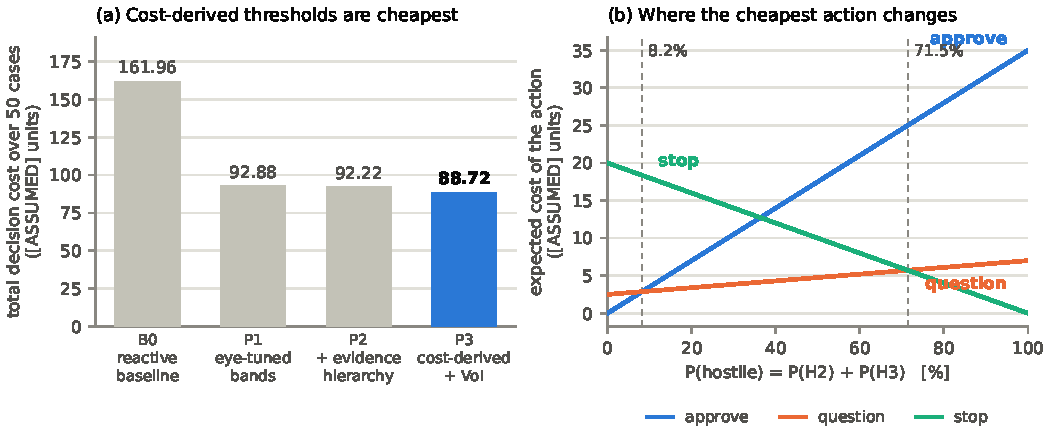
\includegraphics[width=\columnwidth]{figures/results.pdf}
\caption{(a) Total decision cost over the 50-case set; lower is better. (b) Expected cost of
each action as belief in a hostile state varies, for a \$19.99 consumable. The dashed lines
mark where the cheapest action changes: these are the derived boundaries, and they replace
the hand-tuned bands. All units are [ASSUMED].}
\label{fig:results}
\end{figure}

\begin{table}[t]
\centering
\small
\begin{tabular}{lrrrr}
\toprule
& \textbf{B0} & \textbf{P1} & \textbf{P2} & \textbf{P3} \\
\midrule
Total decision cost      & 161.96 & 92.88 & 92.22 & \textbf{88.72} \\
False positives          & 0 & 2 & 2 & \textbf{1} \\
False negatives          & 5 & 1 & 1 & 2 \\
Effective false negatives& 5 & 3 & 3 & 3 \\
Intervention precision   & --- & 0.67 & 0.67 & \textbf{0.75} \\
Hostile recall           & 0.00 & 1.00 & 1.00 & 1.00 \\
Human-review rate        & 0\% & 4\% & 2\% & 2\% \\
\bottomrule
\end{tabular}
\caption{Policy comparison over 50 simulated cases, seed 17. Costs in [ASSUMED] units. Over 300 seeds the mean totals are B0 148.83, P1 77.74, P2 83.87, P3 69.30 --- note that P1 and P2 exchange places once the single-draw noise is removed.}
\label{tab:results}
\end{table}

Table~\ref{tab:results} and Figure~\ref{fig:results} give the comparison. The cost-derived
policy is cheapest and simultaneously least intrusive: it has the fewest false positives
and the best intervention precision while matching hostile recall. It repairs two decisions
in which the hand-tuned bands challenged small purchases for less than the cost of the
challenge.

\paragraph{The margin is concentrated, not general.} The entire advantage over the baseline
comes from the two hostile cases. On the 45 legitimate cases alone the baseline wins
outright, 0.00 against 4.00, because it never pays friction or review costs. This is the
honest form of the result and it is why cost, not accuracy, is the reported metric.

\paragraph{Over 300 seeds the headline holds and the fine ranking does not.}
Table~\ref{tab:results} is one draw. Repeating the whole pipeline over 300 seeds, P3 is
cheaper than the reactive baseline in \textbf{99.3\%} of them, with a mean margin of 79.53
(5th--95th percentile 21.75--141.00); seed 17's margin of 73.24 sits at the 45th
percentile, so it is typical rather than favourable. But P3 is cheapest \emph{of all four
policies} in only \textbf{61.0\%} of seeds, so the correct claim is a tendency with a win
rate, not a property. More sharply, the single-seed run reported the practitioner-derived
hard rule as a small saving (P2 92.22 against P1 92.88); across 300 seeds that ordering
reverses, with mean P1 77.74 against P2 83.87. The constraint costs \textbf{6.13 units on
average} and wins in 49.0\% of seeds. We report it as a price paid deliberately for a
fairness property---not escalating on device evidence alone---rather than as a free
improvement, which is what a single seed made it look like.

\paragraph{The loss ratio forbids aggressive blocking.} For a \$19.99 consumable a wrong
approval costs 34.99 and a wrong refusal 19.99 under our assumed matrix, a ratio of about
1.75:1. Evaluating Equation~\ref{eq:argmin} places the refusal boundary at 71.5\% and the
challenge boundary at 8.2\%, against hand-tuned bands of 5\%, 25\% and 60\%. We note the
contrast with payment-fraud settings, where much larger asymmetries are reported and
correspondingly low thresholds follow; we have no citable figure for that comparison and
state it as context rather than as evidence. Within our assumptions the practitioners'
rejection of purchase-time gating has a quantitative form---and the ratio is itself an
assumption, taking values 0.40, 1.43 or 1.75 across the price points and penalties
examined below.

\paragraph{Sensitivity to a contested cost.} A practitioner disputed our assumed
chargeback penalty on the grounds that the platform is merchant of record and the
developer's exposure is bounded by the revenue. Setting that penalty to zero moves the
refusal boundary from 71.5\% to 81.4\% for a \$19.99 consumable and to 91.6\% for a \$4.99
one, where the ratio inverts to 0.40---a wrong refusal then costs more than twice a wrong
approval. (These boundaries, like those above, are the argmin crossings of
Equation~\ref{eq:argmin}, not values of Equation~\ref{eq:twoaction}.) The policy ranking is
unchanged (B0 131.96, P1 92.88, P2 88.47, P3 80.97) and one action in fifty differs. The
disputed parameter determines where the boundary sits, not which policy wins. The only
configuration retaining an adverse ratio at zero penalty is the high-value consumable, at
1.43---the single corner in which blocking can pay.

\paragraph{Information is rarely worth buying at purchase time.} With review priced at 9.40,
value of information exceeded the fee in one case of fifty. In the most genuinely ambiguous
case in the set, where no state exceeded 38\% belief, VoI was 7.52 against that fee: the
model declines to buy the review. A practitioner reached the same conclusion from
experience, observing that the resolving evidence is days away. Two independent routes, one
answer.

\paragraph{Informative is not actionable.} Ranked from the priors, the highest information
gain belongs to session type and device age (0.095 bits each)---the two features the
practitioner-derived hard rule forbids escalating on. At the ambiguous case above, the
top-ranked purchasable check is an account email-change check at 0.332 bits, which is
exactly the evidence that resolved that case in our decision record. A zero-gain control
scores 0.000 as required.

\section{Failure Analysis}
\label{sec:failures}

Six incorrect or degraded decisions were examined and named, each attributed to the layer
that produced it: costs (L0), the set of possible worlds (L1), the local base rates (L2),
the shape of the answer (L3), or the action rule (L4).

\textbf{F1, the invisible abuser (L4).} A refund-abuse case was approved by every policy.
The decision variable is $p_{\text{hostile}}$, which by construction cannot see $H_5$. The
defect is the choice of event, not the threshold.

\textbf{F2, the futile challenge (L0).} A family-member case was challenged at a cost of
36.0 against 32.0 for approving. A challenge cannot separate states in which the real
cardholder is present, so the policy paid the full loss plus friction.

\textbf{F3, the clean-account takeover (L4).} An account takeover on an established account
carried no account-level risk signal, so the hard rule capped escalation at a challenge.
This is the predicted cost of the practitioner constraint, and the evidence planner
quantifies it: the check that would have resolved the case is the one the rule forbids
acting upon.

\textbf{F4, friction on the faithful (L2).} A legitimate purchase crossed the challenge
boundary because a direct-to-store session and an empty purchase history were treated as
independent evidence. The defect is in the belief, not the boundary.

\textbf{F5, the amount-blind band (L4), repaired.} Hand-tuned bands challenged a \$4.99
purchase for more than the challenge could save. The cost-derived policy approves it. The
failure is retained because it demonstrates the repair: a derived boundary moves with the
stake, a fixed band does not.

\textbf{F6, the belief-blind refund grant (L1/L3).} The refund-abuse case later requested a
refund with 99\% of the item consumed---the defining signature of the abuse---and the agent
still preferred granting it, because consumption magnitude is read by one rule but never
given a likelihood. An observed quantity with no place in the world model cannot influence
a belief. This gap was found by the simulation, not anticipated.

\paragraph{Highest-cost error.} Approving a hostile purchase of a high-value consumable,
realised by the baseline at 64.99 units. It is worst because it is irreversible: a consumed
item cannot be revoked, unlike a subscription or permanent unlock, so no later correction
recovers any part of the loss.

\section{Limitations, Ethics, and Human Control}
\label{sec:limitations}

\paragraph{The model is cleaner than the problem.} Our sharpest limitation was identified by
both a practitioner and an adversarial review of this work: the agent treats human review as
an oracle that resolves the hidden state, when in production no reviewer can resolve a
stolen-card case at purchase time, because the resolving evidence arrives days later. Part
of the reported advantage of the cost-derived policy is therefore an artefact of an action
the modelled reviewer can perform and a real one cannot. The system is properly an
asynchronous state machine over platform events, not the synchronous decision loop modelled
here.

\paragraph{The product-split claim was nearly circular, and the sweep rescues it.} In the
reported 50-case draw, all five non-legitimate cases are consumables. A conclusion that
gating's value concentrates in consumables cannot be supported by a batch that never
generated a hostile subscription or permanent unlock, and we quoted that conclusion to a
practitioner while eliciting DC-13, DC-14 and DC-16. The seed sweep supplies what the
single draw could not: that all-consumable configuration arises in only 14.3\% of seeds, and
across the 54.7\% of seeds containing at least one hostile case on a revocable product the
mean margin over the baseline falls to 68.95, against 92.28 where every hostile case is a
consumable. The direction of the claim survives; the single-seed evidence for it did not.

\paragraph{The surface we argue matters is the one we barely measured.} The consumption
response is, on our own argument, the uncontested and more valuable decision surface. It is
exercised by 2 of 50 cases and no metric is reported for it. The paper therefore evaluates
the surface it concludes is contested and does not evaluate the surface it recommends. A
refund-stage case set is the first thing the next version needs.

\paragraph{Prior population.} The priors describe accounts, while the agent scores
transactions, and hostile states emit purchases in bursts. The per-transaction hostile rate
is therefore structurally higher than the per-account rate we used. This is the base-rate
error in its classic form and it affects every number downstream.

\paragraph{Assumed parameters and simulated data.} Every prior, likelihood and cost is an
explicit assumption. We did not locate public base rates for in-app purchase fraud in
searches of academic databases and platform documentation during August 2026; we do not
claim none exist. Cases are
drawn from the same likelihood tables the agent uses, so the belief update is correctly
specified by construction and real posteriors would be worse. Calibration on such data is
structurally uninformative: with 50 cases and two hostile ones it demonstrates procedure
only.

\paragraph{Modelling gaps.} Correlated evidence is double counted. At least one world is
missing---purchase for grey-market resale, which is behaviourally distinct from the states
we model. The action space excludes the rate-limited grant a practitioner proposed. The
platform action space is wider than the three refund preferences we modelled, including a
prorated option we cannot express. Infrastructure failure is unmodelled: notifications are
at-least-once and may be missed, which we know first-hand from the defect described in
Section~\ref{sec:related}.

\paragraph{Selective labels and adaptation.} Blocked-but-legitimate cases are never
observed, so the evaluation set is systematically incomplete in the field. Worse, a
deployed policy changes the population it observes: attackers adapt to thresholds and
legitimate users adapt to friction, so a calibrated policy decays.

\paragraph{Ethics and human control.} False positives fall on people, not on a metric. The
costs we assign to a wrong refusal understate the reality: support contact, account
recovery and repeated authentication are borne by the customer. Two groups deserve explicit
protection. Families and children are the most likely cause of an ``unintended purchase''
claim, and a stated refund reason is not evidence of fraud; such cases must route to a
disputed-purchase pathway rather than to enforcement. Second, a persistent device signal
that survives reinstallation---valuable precisely because it cannot be erased---can follow
a device to an innocent later owner, and must therefore carry a reason, a timestamp, a
decay policy, and an appeal route. More generally, the agent's output at the refund surface
is advisory: the platform decides, and the agent contributes information. A system that
quietly converts a probability into an unappealable penalty has exceeded its warrant, and
no threshold should be permitted to override a hard rule set by a human.

\section{Conclusion and New Questions}

An entitlement decision under hidden intent is a small, well-posed decision problem, and
treating it explicitly---beliefs, costs, and boundaries derived rather than chosen---is
both cheaper than a hand-tuned policy and easier to defend than a black box. The
substantive finding is not the ranking of policies but the size of the loss ratio: at
roughly 1.75:1, and plausibly lower, this domain does not support aggressive blocking, and
the practitioners who told us so were right for a reason we can now state numerically.

Four questions follow. What is the per-transaction hostile base rate, given that hostile
accounts emit bursts? What does a rate-limited grant cost, and does it dominate both
blocking and unconditional granting? How should an agent behave when the informative
signals are ones it is forbidden to act on? And how quickly does a published threshold
decay once the population adapts to it?

\section*{AI Use Statement}

AI assistance was used throughout this project and its contribution is stated here in full.
An AI assistant helped compile technical terminology and search queries for the research
file, drafted and refined the Reddit questions, implemented and revised the simulation code,
generated the figure, and drafted this manuscript. Three adversarial AI reviews
(practitioner, probability, and preprint) were run against the artefacts; their comments
were accepted or rejected individually with recorded reasoning, and one review's headline
claim was rejected after being tested directly against the code. All design decisions,
every accept/reject judgement on review comments, all public discussion in the author's own
words, and responsibility for the contents of this paper are the author's. Factual claims
about platform behaviour were verified against primary documentation rather than accepted
from an AI assistant; one such check corrected an error in our own design record. Numeric
results were produced by executing the code, not by an AI assistant reporting them.

\section*{Contribution Statement}

Single-author work. Problem selection, all public discussions, agent design, software
development, tests, citation checks, preprint sections, and PDF checks were carried out by
the author with the AI assistance described above.

\section*{Reproducibility}

Code, data, the discussion record, the decision record and the review record are available
at \url{https://github.com/SL-A-SH/AI-Native-Cohort/tree/master/week1/deliverables/student-project}. The
random seed is fixed; \texttt{python src/simulator.py} reproduces every number reported
here.

% `named` ships with the IJCAI kit; `plain` is the drafting fallback.
\ifnum\usingijcai=1\bibliographystyle{named}\else\bibliographystyle{plain}\fi
\bibliography{references}

\end{document}
